\documentclass[parskip,10pt,abstracton]{scrartcl}
\usepackage[top=3cm, bottom=3cm, left=3cm, right=3cm]{geometry}
\usepackage{polyglossia}
\setmainlanguage{german}
\pagenumbering{gobble}

\usepackage{setspace}
\onehalfspacing

% ------------------------------------------------------------------------------------
% packages
\usepackage{graphicx}
\usepackage{tikz}
\usetikzlibrary{arrows,shapes,positioning, shadows,trees}
\usepackage{enumerate}

% ------------------------------------------------------------------------------------
% Header
% ------------------------------------------------------------------------------------
\renewcommand*{\maketitle}{%
	{\centering\LARGE\sffamily\bfseries Aufgabe 3: Strukturierung der Nutzeroberfläche \par}
	\vspace{3em}
}

% ====================================================================================
% Document
% ====================================================================================
\begin{document}

\maketitle

% ------------------------------------------------------------------------------------
\section*{Entwurf 1} % Chris 1

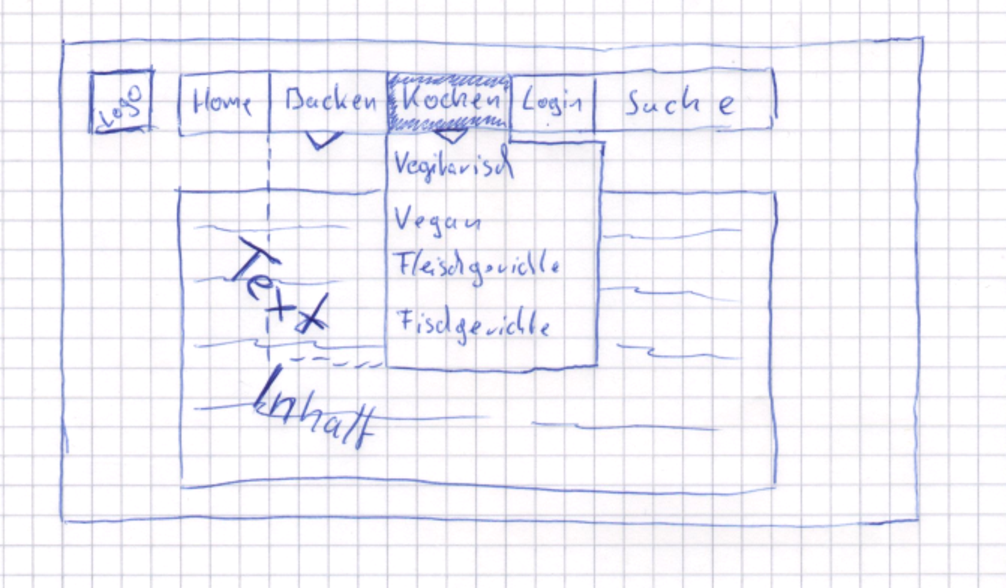
\includegraphics[scale=0.8]{Entwürfe/Chris/chris1.pdf}


\textbf{Vorteile:} \\
- einfach und übersichtlich\\
- Seite nicht überladen\\
- viel Platz für Inhalt

\textbf{Nachteile:} \\
- Menüpunkte Backen/Kochen können unübersichtlich werden bei zu vielen Unterkategorien\\
- unklar, was Login beinhaltet (welche Funktionen hat man davon?) -> Hinweis auf persönliche Funktionen / Möglichkeiten

% ------------------------------------------------------------------------------------
\section*{Entwurf 2} % Chris 2

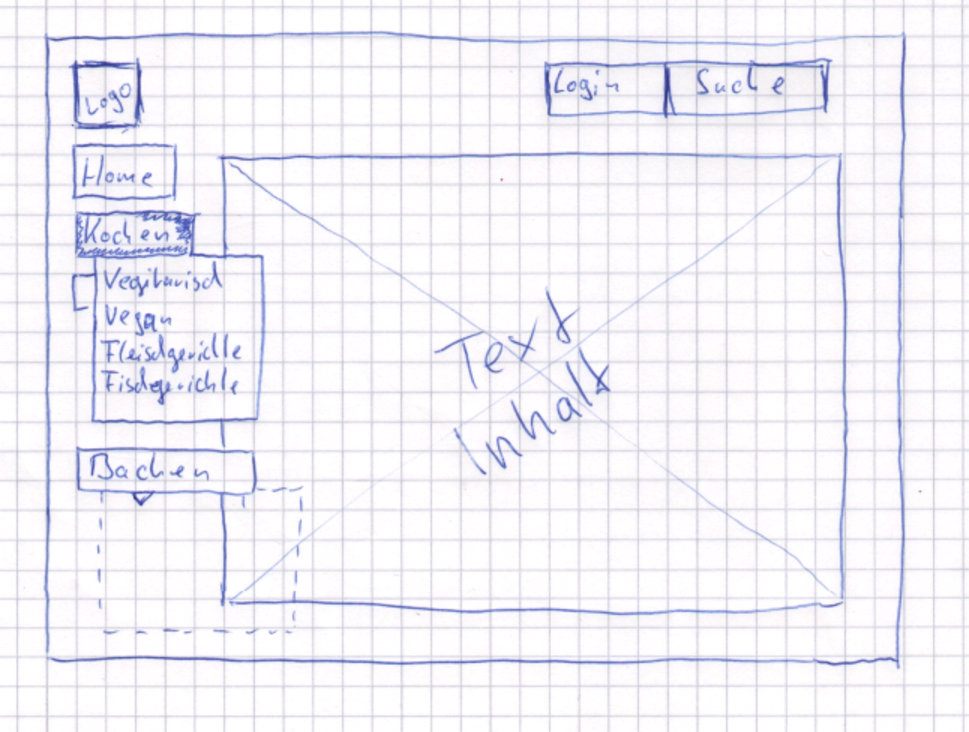
\includegraphics[scale=0.8]{Entwürfe/Chris/chris2.pdf}

\textbf{Vorteile:}\\
- klassischer Aufbau und daher intuitives Zurechtfinden möglich (Position von Login und Suche) \\
- übersichtliches Menü, das sich anpasst (Ein- und Ausklappen möglich).
-

\textbf{Nachteile:}\\
- Seitenmenü kann problematisch werden, wenn Menüpunkte zu lang sind.\\
- nicht innovativ, da es sehr oft verwendet wird.


% ------------------------------------------------------------------------------------
\section*{Entwurf 3} % Velat 1

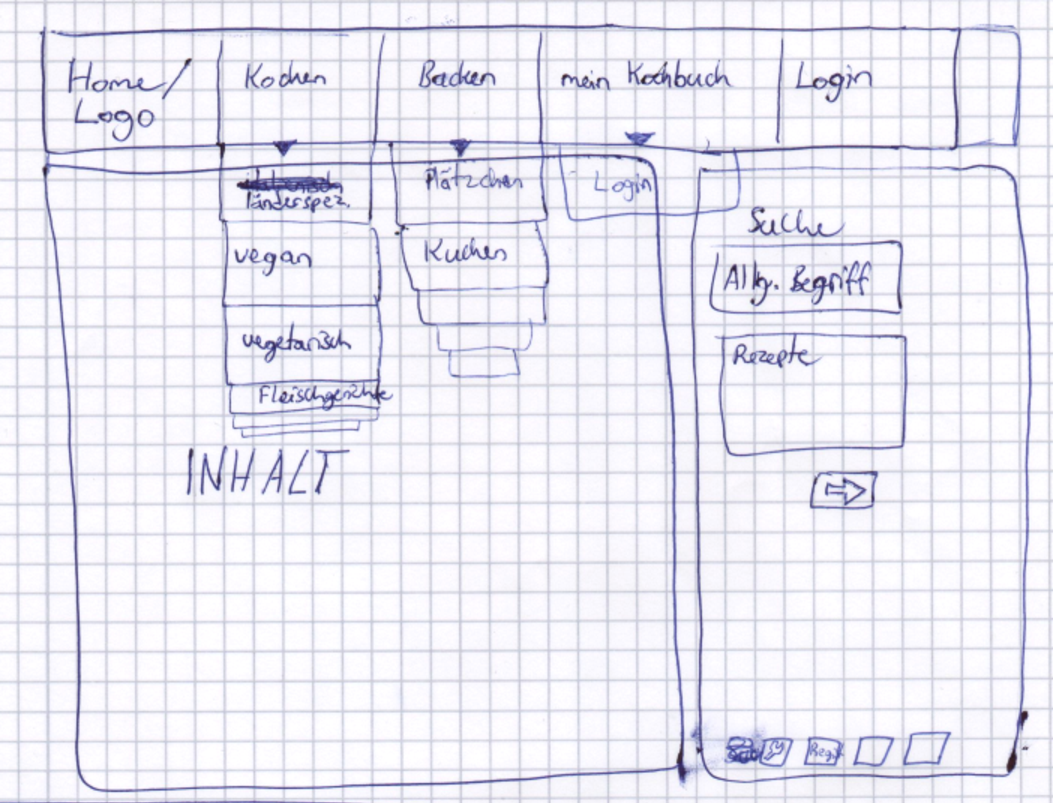
\includegraphics[scale=0.8]{Entwürfe/Velat/velat1.pdf}


\textbf{Vorteile:}\\
- es ist ersichtlich, dass es einen eigenen Kochbuchbereich gibt, für den man sich einloggen muss.\\
- innovativer Suchbereich\\
- Suchbereich als eigener Frame jederzeit sichtbar


\textbf{Nachteile:}\\
- Menüpunkte haben zu viele Unterpunkte im Dropdownmenü\\
- Suchbereich verbraucht Platz von Inhaltsseite\\
- Suchfunktion zu kompliziert

% ------------------------------------------------------------------------------------
\section*{Entwurf 4} % Velat 2

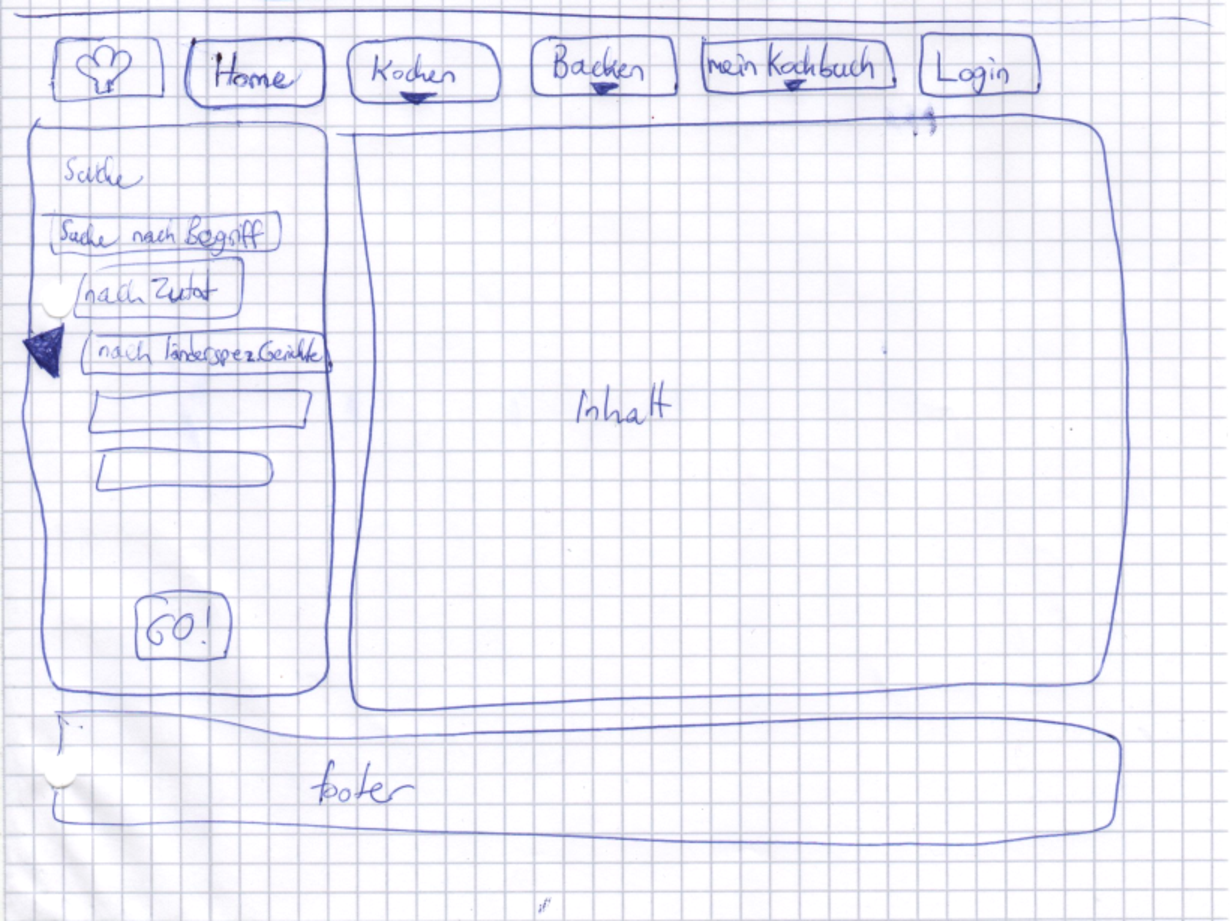
\includegraphics[scale=0.8]{Entwürfe/Velat/velat2.pdf}


\textbf{Vorteile:}\\
- seitlicher Suchbereich: Kategorien können aus- und eingeklappt werden: übersichtlich\\
- mehr Platz für Inhalt, da Suchbereich verborgen werden kann.

\textbf{Nachteile:}\\
- Im Dropdownmenü ist persönl. Bereich schon enthalten, obwohl noch nicht eingeloggt.

\newpage
% ------------------------------------------------------------------------------------
\section*{Entwurf 5} % Tamar 1

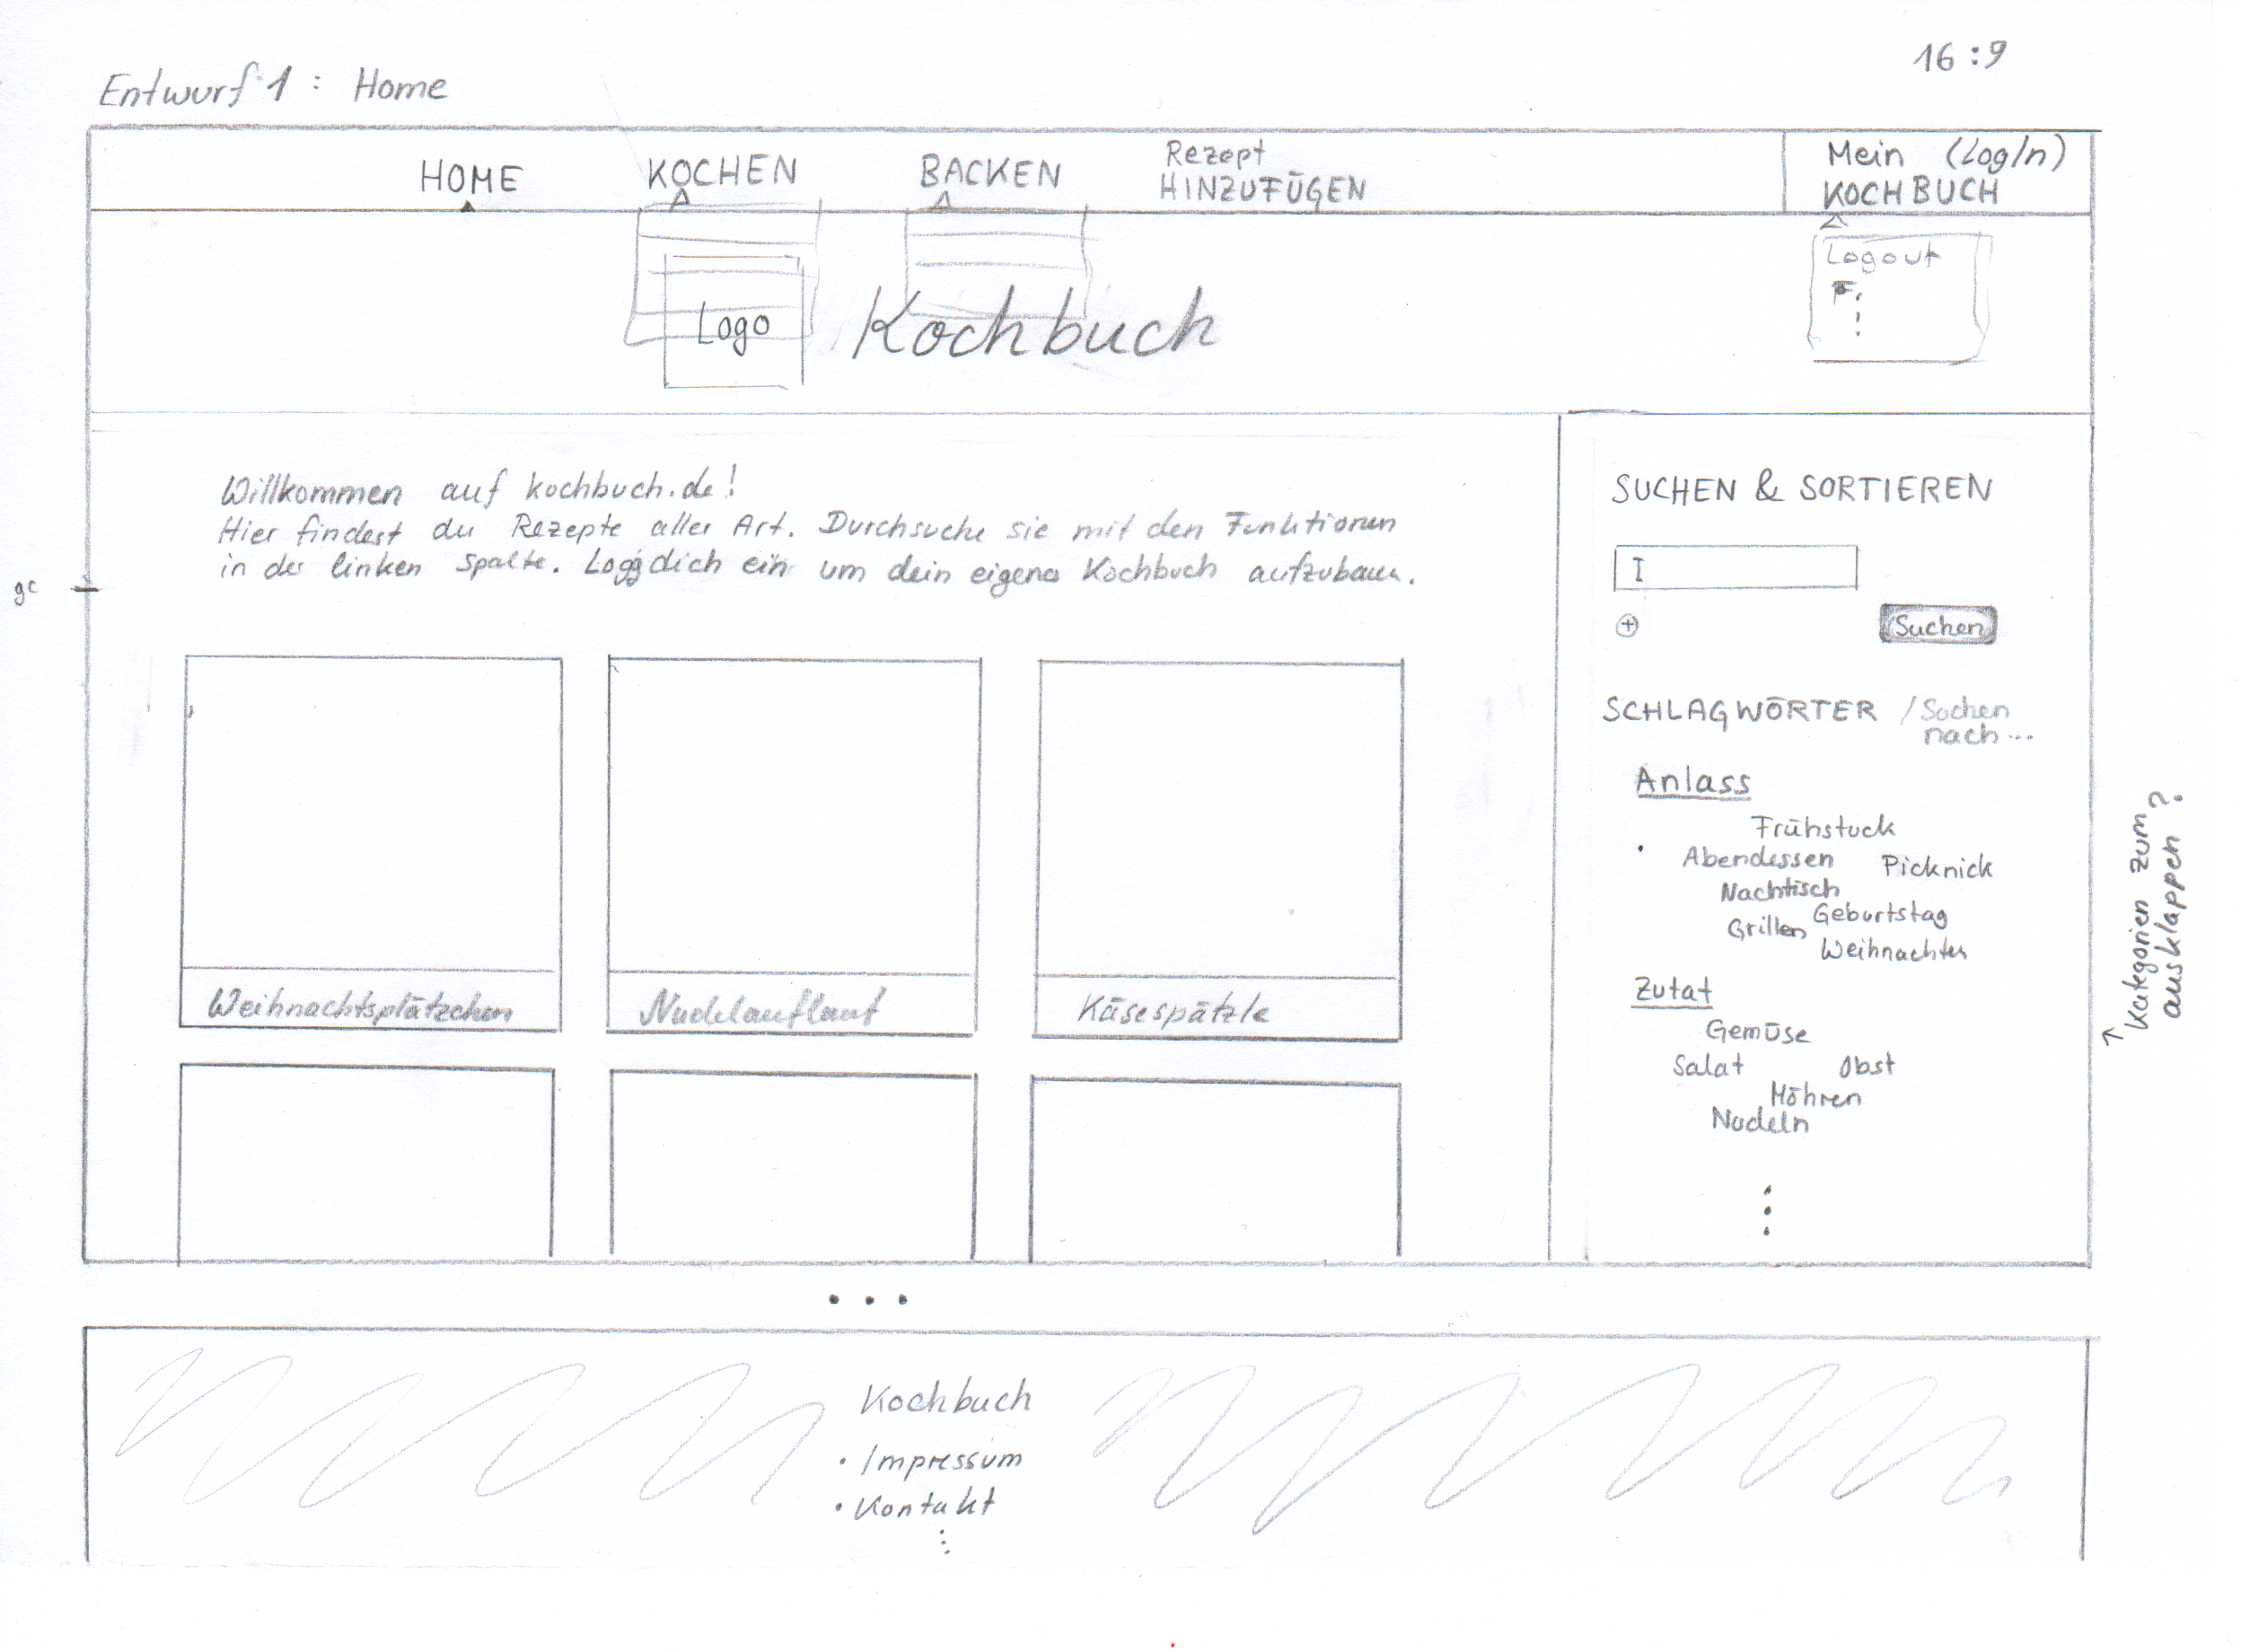
\includegraphics[scale=2.5]{Entwürfe/Tamar/entwurf1.1_home.png}
%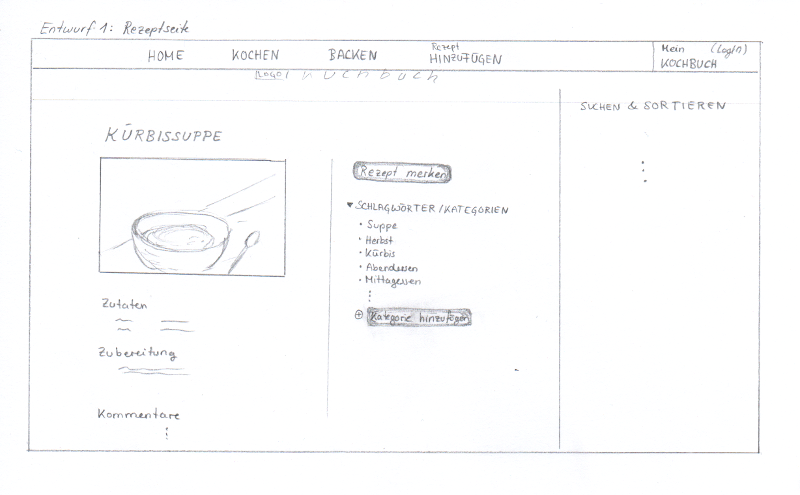
\includegraphics[scale=0.4]{Entwürfe/Tamar/entwurf1.2_rezeptseite.png}\\
%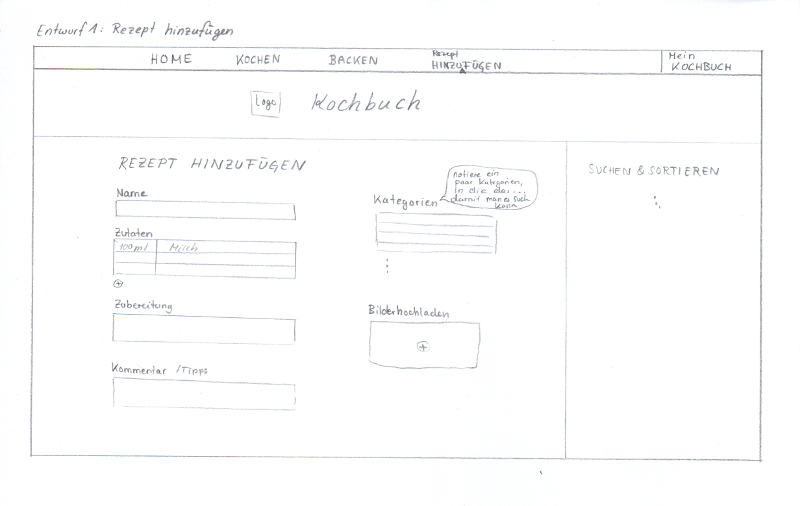
\includegraphics[scale=0.4]{Entwürfe/Tamar/entwurf1.3_hinzufügen.png}



\textbf{Vorteile:}\\
- klassischer Aufbau\\
- Suche jederzeit sichtbar\\
- übersichtlich

\textbf{Nachteile:}\\
- Rezept hinzufügen sollte unter mein Kochbuch kommen, da es sonst nicht in die Navigationsstruktur passt\\
- Suchfunktion verbraucht Platz\\
- auf Rezeptseite muss Rezept mehr Platz einnehmen
\newpage
% ------------------------------------------------------------------------------------
\section*{Entwurf 6} % Tamar 2

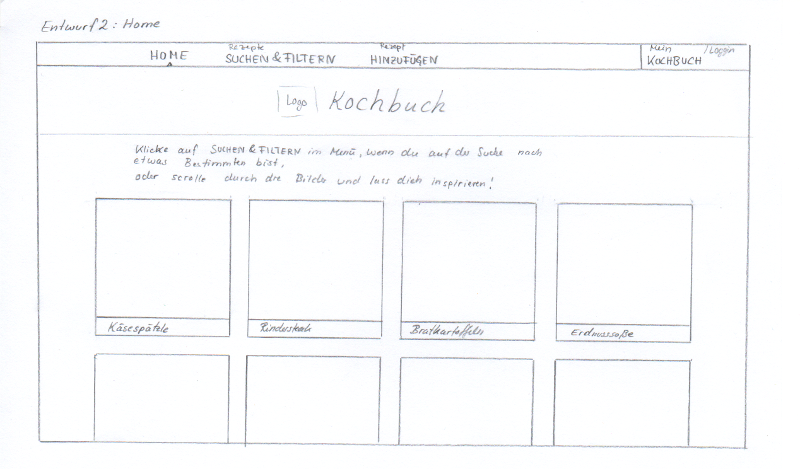
\includegraphics[scale=2.5]{Entwürfe/Tamar/entwurf2.1_home.png}
%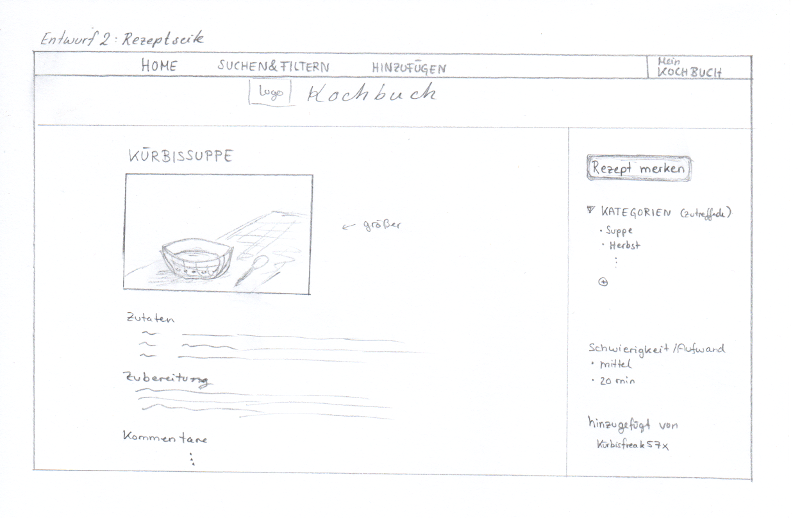
\includegraphics[scale=0.4]{Entwürfe/Tamar/entwurf2.2_rezeptseite.png}\\
%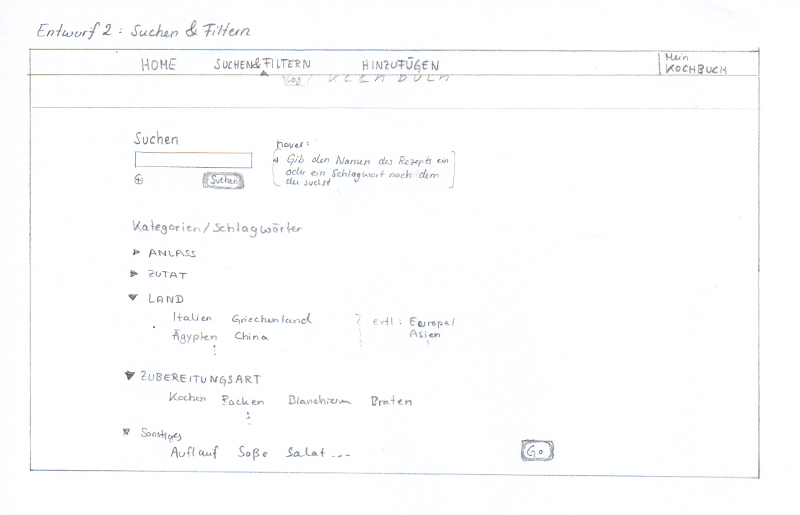
\includegraphics[scale=0.4]{Entwürfe/Tamar/entwurf2.3_filtern1.png}
%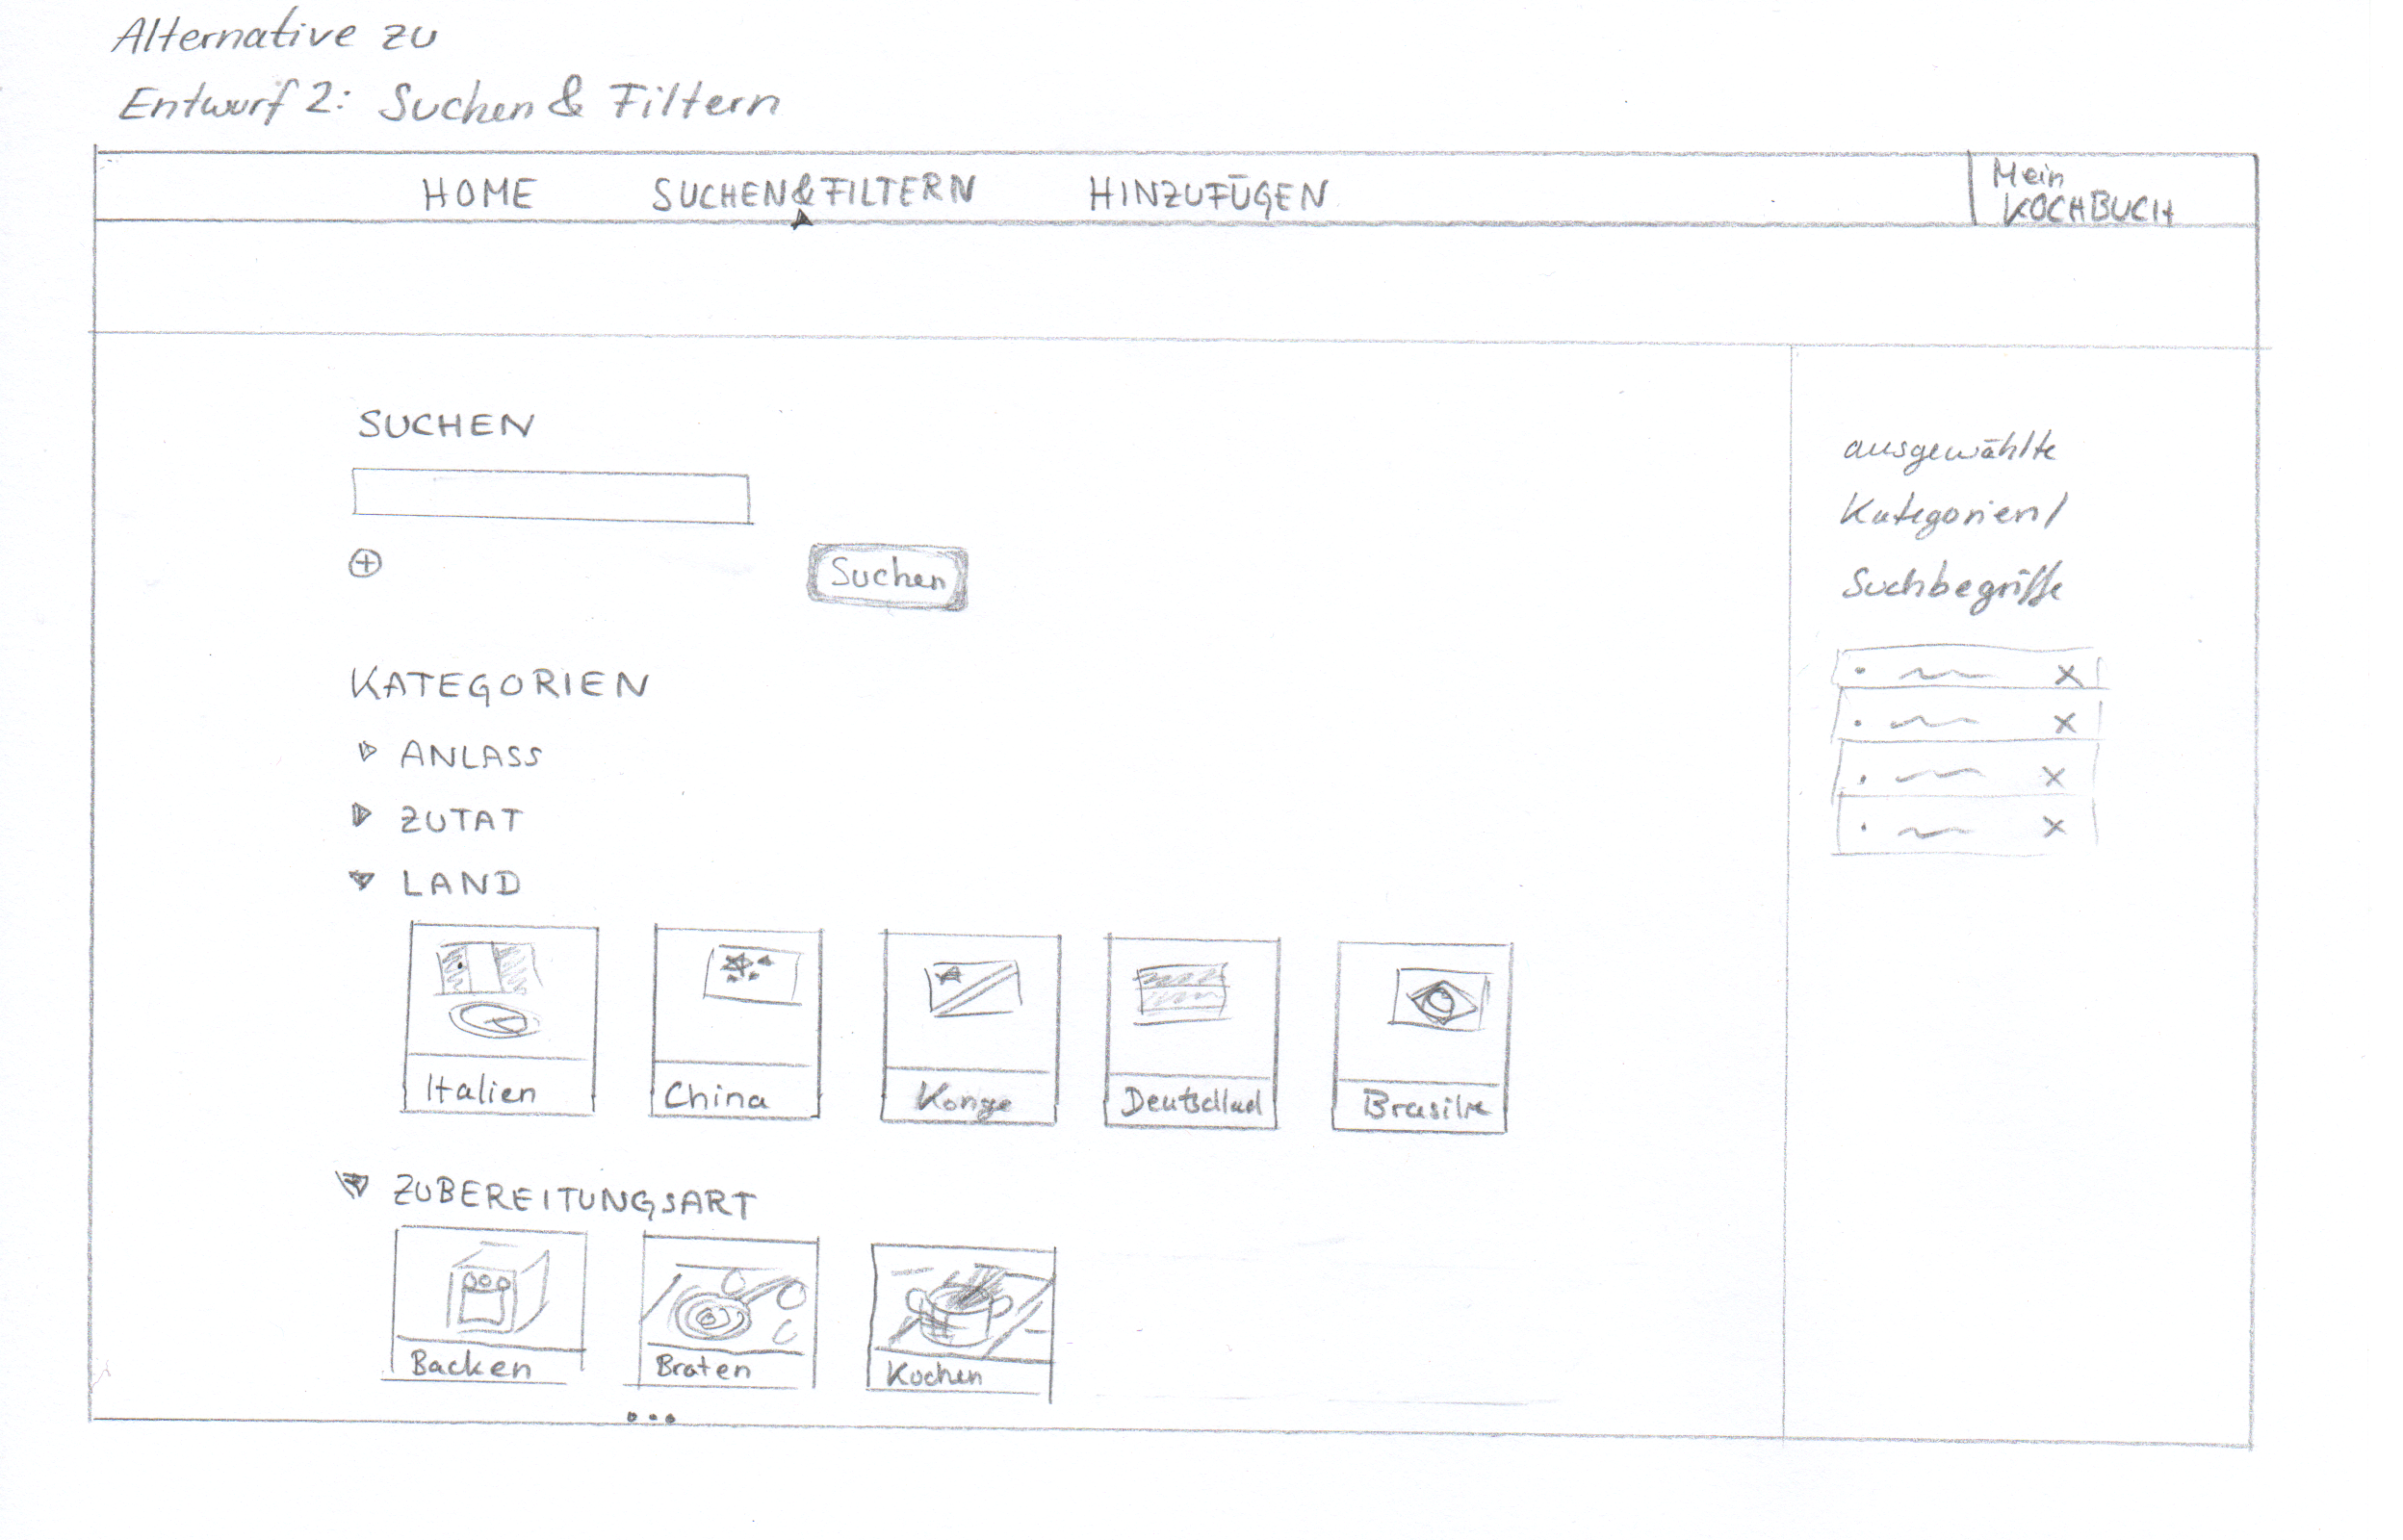
\includegraphics[scale=0.4]{Entwürfe/Tamar/entwurf2.3_filtern2.png}


\textbf{Vorteile:} \\
- mehr Platz\\
- aufgeräumter

\textbf{Nachteile:}\\
- Suche als eigene Seite hat Nachteil, dass man ausgewählte Kategorien nicht nebenher sieht.\\
- Suchseite zu überladen


\newpage
% ------------------------------------------------------------------------------------
\section*{Planung des Prototypen}

\begin{enumerate}
 \item möglichst übersichtliches, klassisches Design um intuitives Zurechtfinden zu ermöglichen (rechts oben Login)
 \item Navigation aufgespalten:
 \begin{itemize}
  \item einerseits: horizontale Navigation stellt organisatorisches dar: Meta-Navigation, wie Home und Profilverwaltung / persönlicher Bereich
  \item andererseits: Seitenmenü enthält Kategorien, nach denen Rezepte sortiert/gefiltert werden können. Für Nutzer, die genau wissen was sie wollen, gibt es die Suchleiste.
 \end{itemize}
 \item Navigation und Struktur der Webseite ist für den Nutzer ersichtlich, da auf jeder Seite Navigation an gleicher Stelle bleibt und sich eventuell dynamisch anpasst (checkboxen)
 \item Navigation nimmt nicht notwendigerweise zu viel Platz der Webseite ein, da sie eingeklappt/verborgen werden kann
 \item Damit das seitliche Menü ersichtlich bleibt, sind einzelne Kategorien (Kochen, Backen, usw.) eingeklappt. Nach Bedarf können diese ausgeklappt werden, damit Unterkategorien sichtbar sind. 
 \item Der Großteil des Seiteninhalts besteht aus Bildern von Rezepten und der dazugehörige Kochvorgang.

\end{enumerate}


\end{document}



